\RequirePackage{plautopatch}
\documentclass[dvipdfmx,a4paper]{jsarticle}
\usepackage{graphicx}
\usepackage{amsmath}
\usepackage{amssymb}
\usepackage{float}
\usepackage{wrapfig}

\title{船体運動力学 課題 2}
\author{古賀 光一朗}
\date{2025年6月23日 ~ 2025年6月30日}

\begin{document}

\maketitle
$$\text{提出期限:2025 年 6 月 30 日(月)10:30AM}$$
---
\begin{wrapfigure}{r}{0.4\linewidth} % 横幅を調整
\vspace{-20pt} % 上方向の余白を調整
\centering
% ご自身の画像ファイル名に合わせてパスを修正してください
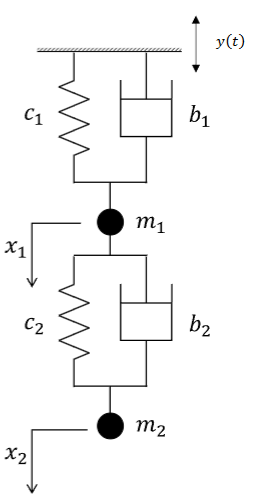
\includegraphics[width=\linewidth]{summer/ship-dynamics/day2_rensei.png} 
\caption{連成したばね-マス-ダッシュポット系}
\label{fig:damper-system}
\end{wrapfigure}
右図の連成したばね-マス-ダッシュポット系の支持部(天井)が
\begin{equation}
 y(t)=a\cos{\omega t}
\end{equation}
で定常的に強制動揺されている。なお、システムは線形であり、上下運動しかしない。減衰力は振動減衰を行う程度に小さいとする(過減衰ではない)。

(1-1)質点の無次元化された運動方程式が
\begin{equation}
    \begin{gathered}\ddot{\hat x}+2\Gamma\dot{\hat x}+D\hat x=\Gamma\prime\dot{\hat y}+D\prime\hat y\end{gathered}\\
\end{equation}
で表されるという。このときの$\Gamma, D, \Gamma\prime,D\prime $を数式で示しなさい。


ただし、無次元化は $t=T\hat t , \space x=X\hat x, \space y=X\hat y$ であり、変位ベクトルは次の通りに与える。
$$x=\begin{Bmatrix}x_1\\x_2\end{Bmatrix},y=\begin{Bmatrix}y\\0\end{Bmatrix}$$


まず、質点$m_1$および$m_2$の運動方程式をニュートンの運動法則に基づいて立式する。変位$x_1, x_2$は鉛直下向きを正とする。

質点$m_1$に作用する力は、
\begin{itemize}
    \item ばね $c_1$ からの復元力: $-c_1 (x_1 - y)$
    \item ダンパ $b_1$ からの減衰力: $-b_1 (\dot{x}_1 - \dot{y})$
    \item ばね $c_2$ からの復元力: $-c_2 (x_1 - x_2)$
    \item ダンパ $b_2$ からの減衰力: $-b_2 (\dot{x}_1 - \dot{x}_2)$
\end{itemize}
よって、$m_1$の運動方程式は次式となる。
\begin{equation}
    m_1 \ddot{x}_1 = -c_1 (x_1 - y) - b_1 (\dot{x}_1 - \dot{y}) - c_2 (x_1 - x_2) - b_2 (\dot{x}_1 - \dot{x}_2)
\end{equation}
整理すると、
\begin{equation}
    m_1 \ddot{x}_1 + (b_1 + b_2) \dot{x}_1 - b_2 \dot{x}_2 + (c_1 + c_2) x_1 - c_2 x_2 = b_1 \dot{y} + c_1 y \label{eq:m1}
\end{equation}

次に、質点$m_2$に作用する力は、
\begin{itemize}
    \item ばね $c_2$ からの復元力: $c_2 (x_1 - x_2)$
    \item ダンパ $b_2$ からの減衰力: $b_2 (\dot{x}_1 - \dot{x}_2)$
\end{itemize}
よって、$m_2$の運動方程式は次式となる。
\begin{equation}
    m_2 \ddot{x}_2 = c_2 (x_1 - x_2) + b_2 (\dot{x}_1 - \dot{x}_2)
\end{equation}
整理すると、
\begin{equation}
    m_2 \ddot{x}_2 - b_2 \dot{x}_1 + b_2 \dot{x}_2 - c_2 x_1 + c_2 x_2 = 0 \label{eq:m2}
\end{equation}

式 \eqref{eq:m1}, \eqref{eq:m2} を行列・ベクトル形式で表現する。変位ベクトルを $x = \begin{Bmatrix} x_1 & x_2 \end{Bmatrix}^T$ とすると、
\begin{equation}
    M \ddot{x} + C \dot{x} + K x = F(t)
\end{equation}
ここで、各行列およびベクトルは以下の通りである。
\begin{gather}
    M = \begin{bmatrix} m_1 & 0 \\ 0 & m_2 \end{bmatrix}, \quad
    C = \begin{bmatrix} b_1+b_2 & -b_2 \\ -b_2 & b_2 \end{bmatrix}, \quad
    K = \begin{bmatrix} c_1+c_2 & -c_2 \\ -c_2 & c_2 \end{bmatrix} \\
    F(t) = \begin{Bmatrix} b_1 \dot{y} + c_1 y \\ 0 \end{Bmatrix} = \begin{bmatrix} b_1 & 0 \\ 0 & 0 \end{bmatrix} \begin{Bmatrix} \dot{y} \\ 0 \end{Bmatrix} + \begin{bmatrix} c_1 & 0 \\ 0 & 0 \end{bmatrix} \begin{Bmatrix} y \\ 0 \end{Bmatrix}
\end{gather}
外力項 $F(t)$ は、支持部の変位 $y(t)$ を用いて $F(t) = C' \dot{y} + K' y$ と書ける。ただし、$y$ はベクトル $y=\begin{Bmatrix}y & 0\end{Bmatrix}^T$ とする。

次に、与えられた定義 $t=T\hat t , \space x=X\hat x, \space y=X\hat y$ を用いて無次元化を行う。時間微分は以下の関係となる。
$$ \dot{(\cdot)} = \frac{d}{dt}(\cdot) = \frac{1}{T}\frac{d}{d\hat{t}}(\cdot) = \frac{1}{T}\dot{\hat{(\cdot)}} $$
$$ \ddot{(\cdot)} = \frac{d^2}{dt^2}(\cdot) = \frac{1}{T^2}\frac{d^2}{d\hat{t}^2}(\cdot) = \frac{1}{T^2}\ddot{\hat{(\cdot)}} $$
これらを運動方程式に代入する。
$$ M \frac{X}{T^2} \ddot{\hat{x}} + C \frac{X}{T} \dot{\hat{x}} + K X \hat{x} = C' \frac{X}{T} \dot{\hat{y}} + K' X \hat{y} $$
両辺を $X$ で割り、左から質量行列の逆行列 $M^{-1}$ を乗じると、
$$ \frac{1}{T^2} \ddot{\hat{x}} + \frac{1}{T} M^{-1} C \dot{\hat{x}} + M^{-1} K \hat{x} = \frac{1}{T} M^{-1} C' \dot{\hat{y}} + M^{-1} K' \hat{y} $$
さらに両辺に $T^2$ を乗じると、
$$ \ddot{\hat{x}} + T M^{-1} C \dot{\hat{x}} + T^2 M^{-1} K \hat{x} = T M^{-1} C' \dot{\hat{y}} + T^2 M^{-1} K' \hat{y} $$
この式を、問題で与えられた無次元化された運動方程式
$$ \ddot{\hat x}+2\Gamma\dot{\hat x}+D\hat x=\Gamma\prime\dot{\hat y}+D\prime\hat y $$
と比較することにより、各係数行列は以下のように求められる。

$M^{-1} = \begin{bmatrix} 1/m_1 & 0 \\ 0 & 1/m_2 \end{bmatrix}$ であるから、
\begin{equation}
    \Gamma = \frac{T}{2} M^{-1}C = \frac{T}{2} \begin{bmatrix} (b_1+b_2)/m_1 & -b_2/m_1 \\ -b_2/m_2 & b_2/m_2 \end{bmatrix}
\end{equation}
\begin{equation}
    D = T^2 M^{-1}K = T^2 \begin{bmatrix} (c_1+c_2)/m_1 & -c_2/m_1 \\ -c_2/m_2 & c_2/m_2 \end{bmatrix}
\end{equation}
\begin{equation}
    \Gamma' = T M^{-1} \begin{bmatrix} b_1 & 0 \\ 0 & 0 \end{bmatrix} = T \begin{bmatrix} b_1/m_1 & 0 \\ 0 & 0 \end{bmatrix}
\end{equation}
\begin{equation}
    D' = T^2 M^{-1} \begin{bmatrix} c_1 & 0 \\ 0 & 0 \end{bmatrix} = T^2 \begin{bmatrix} c_1/m_1 & 0 \\ 0 & 0 \end{bmatrix}
\end{equation}
ここで $T$ は無次元化のための特性時間であり、系の物理定数から任意に定義できる(例: $T = \sqrt{m_1/c_1}$ など)。

(1-2)固有角周波数の大小による運動の特徴を論じなさい。

系の動的な振る舞いを理解するため、外力と減衰を無視した自由振動を考える。運動方程式は $M\ddot{x} + Kx = 0$ となる。解を $x = u e^{i\Omega t}$ と仮定して代入すると、以下の固有値問題を得る。
$$ (K - \Omega^2 M) u = 0 $$
自明でない解 ($u \neq 0$) が存在するためには、係数行列の行列式がゼロでなければならない。
$$ \det(K - \Omega^2 M) = \begin{vmatrix} c_1+c_2 - \Omega^2 m_1 & -c_2 \\ -c_2 & c_2 - \Omega^2 m_2 \end{vmatrix} = 0 $$
これを展開すると、$\Omega^2$ に関する2次方程式が得られる。
$$ m_1 m_2 \Omega^4 - (m_1 c_2 + m_2(c_1+c_2)) \Omega^2 + c_1 c_2 = 0 $$
この方程式の2つの正の解を $\Omega_1^2, \Omega_2^2$ (ただし $\Omega_1 < \Omega_2$)とすると、この系は $\Omega_1$(1次固有角周波数)と $\Omega_2$(2次固有角周波数)という2つの固有角周波数を持つ。

支持部の強制振動の角周波数 $\omega$ と、これらの固有角周波数 $\Omega_1, \Omega_2$ の大小関係によって、系の応答特性は大きく変化する。

\begin{enumerate}
    \item \textbf{共振} \\
    強制振動の角周波数 $\omega$ が、系の固有角周波数 $\Omega_1$ または $\Omega_2$ のいずれかに近づくと、共振現象が発生し、質点の振幅が極めて大きくなる。
    \begin{itemize}
        \item $\omega \approx \Omega_1$ のとき:1次の振動モードが励起される。これは、2つの質点がおおむね同じ方向に(同相で)大きく揺れる運動に対応する。
        \item $\omega \approx \Omega_2$ のとき:2次の振動モードが励起される。これは、2つの質点が互いに逆方向に(逆相で)揺れる運動に対応する。
    \end{itemize}
    減衰が存在するため振幅は有限に留まるが、減衰が小さいほど共振時の振幅は鋭く、大きくなる。

    \item \textbf{低周波数域 ($\omega \ll \Omega_1$)} \\
    加振が非常にゆっくりな場合、慣性力の影響は小さく、系はばねの復元力と外力が釣り合った準静的な状態で運動する。質点 $m_1, m_2$ は支持部の動き $y(t)$ にほぼ追従し、系全体が一体となって動く。振幅応答倍率は1に近くなる。

    \item \textbf{高周波数域 ($\omega \gg \Omega_2$)} \\
    加振が非常に速い場合、質点はその慣性のためにその場に留まろうとし、ほとんど動かなくなる。支持部のみが激しく振動し、質点にはその動きが伝わらない。これは防振(振動絶縁)の効果であり、系の振幅はゼロに近づく。
\end{enumerate}

\end{document}